\documentclass[12pt, a4paper]{article}
\usepackage[print,sort]{standalone}
\usepackage[T1]{fontenc}
\usepackage[utf8]{inputenc}
\usepackage[english]{babel}
\usepackage{graphicx,float}
\usepackage{amssymb}
\usepackage{amsmath,cancel}
\usepackage{mathrsfs}
\usepackage{epstopdf}
\usepackage{subcaption}
\usepackage{slashed}
\usepackage{hhline}
\usepackage[margin=1.2in]{geometry}
\usepackage[hidelinks]{hyperref}
\usepackage{wrapfig}

\begin{document}

\begin{titlepage}
\begin{center}
\vspace*{6cm}
\Huge
\textbf{Project 1} \\
\vspace*{1cm}
\LARGE
FYS4150 - Computational Physics \\ 
\vspace*{10cm}
Even S. Håland 
\end{center}
\end{titlepage}

\section{Introduction}

The purpose of this project is to develop an algorithm that will be used to find a numerical solution 
to the one-dimensional Poisson equation 
\begin{equation}
-u''(x) = f(x), 
\label{poisson}
\end{equation}
where $x\in (0,1)$, with the Dirichlet boundary conditions $u(0)=u(1)=0$. It will be assumed that the 
source term ($f(x)$) takes the form 
\begin{equation}
f(x) = 100e^{-10x}. 
\label{f(x)}
\end{equation}

The solution we obtain numerically will be compared to a closed-form solution given by 
\begin{equation}
u(x) = 1- \left(1-e^{-10}\right)x - e^{-10x}. 
\label{closed-form}
\end{equation}
We can easily show that this is a solution to eq. (\ref{poisson}) by taking the first and second 
derivatives: 
\begin{align*}
    u'(x) & = -\left(1-e^{-10}\right) + 10e^{-10x} \\ 
\Rightarrow \quad  u''(x) & = -100e^{-10x} \\
\Rightarrow \: -u''(x) & = 100e^{-10x} = f(x).  
\end{align*}

The algorithm will be developed in two different stages; first a general one, and then a simplified 
one that deals with the particular problem in this project. The two versions of the algorithm will be 
compared in terms of number of floating point operations and CPU time. 

Another important part of the project is to study the error of the numerical solution, and how it 
evolves as we decrease the step size in the algorithm. Finally we will also solve the equation by using 
library functions, and see why this might not be a good idea. 

\section{Discretization of the Poisson equation}

To solve something numerically we need to make a discrete approximation to the problem. In this case 
we approximate $u(x)$ by $v(x_i)=v_i$, with $x_i=ih$ in the interval $x_0=0$ to $x_{n+1}=1$. The step 
size is defined by $h=1/(n+1)$. The boundary conditions are now given by $v_0 = v_{n+1} = 0$.   

The second derivative is approximated by 
\begin{equation}
u''(x) \approx \frac{v_{i+1} + v_{i-1} - 2v_i}{h^2}, 
\end{equation}
meaning that our problem can be written as 
\begin{equation}
-\frac{v_{i+1} + v_{i-1} - 2v_i}{h^2} = f_i, 
\label{poisson_disc}
\end{equation}
where $f_i = f(x_i)$ and $i=1,\dots,n$. To simplify the expression a little bit we multiply both sides by 
$h^2$, and define $y_i = h^2 f_i$.\footnote{In the project description it is suggested to use 
$\tilde{b}_i = h^2 f_i$, but I found that this can be quite confusing, as $b$ is used to denote 
the diagonal elements of the matrix $\mathbf{A}$, meaning that $\tilde{b}$ is very convenient to use when 
doing the Gauss elimination.}  

Let us now write eq. (\ref{poisson_disc}) explicitly for some values of $i$ (and keep in mind that 
$v_0 = v_{n+1} = 0$): 
\begin{align*}
i = 1 \quad & \Rightarrow \quad -v_2 + 2v_1 = y_1 \\ 
i = 2 \quad & \Rightarrow \quad -v_3 - v_1 + 2v_2 = y_2 \\ 
i = 2 \quad & \Rightarrow \quad -v_4 - v_2 + 2v_3 = y_3 \\ 
\vdots \\
i = n \quad & \Rightarrow \quad  - v_{n-1} + 2v_n = y_n \\ 
\end{align*}
It is now relatively easy to see that this can be written as a matrix equation if we define 
\begin{align*}
\mathbf{v} = \left( \begin{array}{c}
v_1 \\ v_2 \\ \vdots \\ v_n
\end{array} \right) 
\quad \mbox{and} \quad
\mathbf{y} = \left( \begin{array}{c}
y_1 \\ y_2 \\ \vdots \\ y_n 
\end{array} \right) . 
\end{align*}
The equation can then be written as $\mathbf{Av} = \mathbf{y}$, where $\mathbf{A}$ is the 
tridiagonal $n\times n$-matrix given by 
\begin{align*}
\mathbf{A} = \left(\begin{array}{cccccc}
2 & -1 & 0 & \cdots & \cdots & 0 \\ 
-1 & 2 & -1 & 0 & \cdots & \cdots \\ 
0 & -1 & 2 & -1 & 0 & \cdots \\
\cdots & \cdots & \cdots & \cdots & \cdots & \cdots \\              
\cdots & \cdots  & 0 & -1 & 2 & -1 \\ 
0 & \cdots & \cdots & 0 & -1 & 2 \\  
\end{array} \right),  
\end{align*}
meaning that to solve the problem we need to solve this equation for $\mathbf{v}$. 

\section{Developing the algorithm}

When solving a matrix equation we make use of Gaussian elimination. A general tridiagonal matrix can be 
written in terms of vectors $a$, $b$ and $c$ as  
\begin{align*}
\mathbf{A} = \left(\begin{array}{cccccc}
b_1 & c_1 & 0 & \cdots & \cdots & 0 \\ 
a_1 & b_2 & c_2 & 0 & \cdots & \cdots \\ 
0 & a_2 & b_3 & c_3 & 0 & \cdots \\
\cdots & \cdots & \cdots & \cdots & \cdots & \cdots \\              
\cdots & \cdots  & 0 & a_{n-2} & b_{n-1} & c_{n-1} \\ 
0 & \cdots & \cdots & 0 & a_{n-1} & b_n \\  
\end{array} \right), 
\end{align*}
so what we actually want to do is to eliminate all $a$'s in the matrix. We see that to eliminate $a_1$ 
we must multiply the first row by $\frac{a_1}{b_1}$, and then subtract it from the second row, meaning that 
the second row becomes 
\begin{align*}
\left( \begin{array}{cccccc}
0 & b_2 - \frac{c_1 a_1}{b_1} & c_2 & 0 & \cdots & 0 
\end{array} \right). 
\end{align*}
(Notice that the $c$'s are not affected by this procedure.)  
To simplify the expressions we would like to define 
\begin{align*}
\tilde{b}_2 \equiv b_2 - \frac{c_1 a_1}{b_1}.  
\end{align*}
The procedure then continues in the same pattern, and we realize that the new diagonal elements 
($\tilde{b}$'s) can be written as   
\begin{align}
\tilde{b}_i = b_i - \frac{a_i c_{i-1}}{\tilde{b}_{i-1}}. 
\label{btilde}
\end{align}
We must also remember to do the same operations on the right hand side, 
\begin{align}
\tilde{f}_i = y_i - \frac{a_i \tilde{f}_{i-1}}{\tilde{b}_{i-1}}. 
\label{ftilde}
\end{align}

When the elimination is done we need to do a backwards substitution to actually solve the equation for 
each $v_i$. Since we now have a diagonal matrix we should start at the last equation, i.e. 
$\tilde{b}_n v_n = \tilde{f}_n$, which means that 
\begin{align*}
v_n = \frac{\tilde{f}_n}{\tilde{b}_n}. 
\end{align*} 
Now that $v_n$ is known we can move to the second last equation, solve it for $v_{n-1}$, and so on. The 
general expression for $v_i$ becomes 
\begin{align*}
v_i = \frac{\tilde{f}_{i+1} - c_i v_{i+1}}{\tilde{b}_i}.
\label{vi} 
\end{align*}

Before moving on to how I have coded this, and finally look at results, I would like to get all the 
"maths" done by looking at how we in our case can simplify the above expressions.    

\subsection{Simplifying the algorithm}

We have now looked at how the matrix equation is solved when $\mathbf{A}$ is a general tridiagonal matrix. 
However, the matrix we are studying is simplified quite a bit, as all $a_i = c_i = -1$, while 
all $b_i = 2$. The first thing to notice is that eq. (\ref{btilde}) can be written as 
\begin{align*}
\tilde{b}_i = 2- \frac{1}{\tilde{b}_{i-1}}. 
\end{align*}
By writing the first few terms 
\begin{align*}
\tilde{b}_2 = 2 - \frac{1}{2} = \frac{3}{2}, \quad \tilde{b}_3 = 2- \frac{1}{3/2} = \frac{4}{3}, \quad 
\tilde{b}_4 = 2 - \frac{1}{4/3} = \frac{5}{4}, 
\end{align*}
and so on, we realize that we can actually write the $\tilde{b}$'s as 
\begin{align*}
\tilde{b}_i = \frac{i+1}{i}. 
\end{align*}
By doing the same for the $\tilde{f}$'s we find that 
\begin{align*}
\tilde{f}_i = y_i + \frac{i-1}{i}\tilde{f}_{i-1}, 
\end{align*}
and finally 
\begin{align*}
v_{i-1} = \frac{i-1}{i}(\tilde{f}_{i-1} - v_i). 
\end{align*}
When doing these simplifications the total number of floating point operations for each turn in the loop 
is reduced from $6$ to $4$ in the forward substitution, while in the backward substitution the number 
stays the same ($3$). 

\subsection{Coding the algorithm}

At the moment of writing this report I have only written the code in Python, and the code can be found in 
the following git-repository: \vspace{0.5cm} \\ 
\fbox{
\href{https://github.com/evensha/FYS4150/tree/master/Project1}
{https://github.com/evensha/FYS4150/tree/master/Project1} } \vspace{0.5cm} \\ 
The program take two input arguments: 
\begin{enumerate}
\item An argument that specify if we want to run the general or the simplified algorithm ("g" for 
general and "s" for simplified). 
\item The matrix dimension, $n$. 
\end{enumerate}  

When writing the code I have chosen to let all arrays have $n+2$ elements, i.e. $i = 0,1,\dots,n,n+1$, to 
make the arrays correspond to the total number of grid points (including the boundary points), and 
to make the code as close to the mathematical expressions as possible.

After making the necessary arrays ($a$, $b$, $c$, $x$, $f$ and $v$) I make the four different loops, i.e. 
forward and backward substitution in both the general and the simplified way. The loops just update the 
values of the array elements of $b$, $f$ and $v$, meaning that I have chosen not to make separate arrays 
called $\tilde{b}$, $\tilde{f}$, and so on. While running the algorithm I also calculate the CPU time and
number of floating point operations. When the algorithm is done I make an array for the closed form 
solution, and plot it together with the numerical solution from the algorithm, and the (logarithm of) 
the relative error is calculated by the formula
\begin{equation}
\epsilon_i = log_{10}\left(\left| \frac{v_i - u_i}{u_i} \right| \right). 
\label{eq:error}
\end{equation}
All results are shown in the next section. 
   
The last part of the program is to solve the problem by using library functions. I have chosen to use 
functions from the \texttt{scipy} library, which for instance contains the \texttt{lu()}-function for 
LU decomposition, and \texttt{inv()} for inverting a matrix. The CPU time is calculated for this procedure 
as well.  


\section{Results}

Figure \ref{plots} shows the numerical solution plotted together with the closed-form solution for 
$10$, $100$ and $1000$ grid points. When $n=10$ we can see that the numerical estimate is somewhat 
different from the analytical solution, while for $n=100$ and $n=1000$ they seem to be very similar. 
(If one zooms closely in on the $n=100$ plot it is possible to see a slight difference around the 
maximum of the curve, while for $n=1000$ there seems to be no observable difference between the curves.) 

\begin{figure}[ht!]
  \centering
  \begin{subfigure}[b]{0.495\textwidth}
		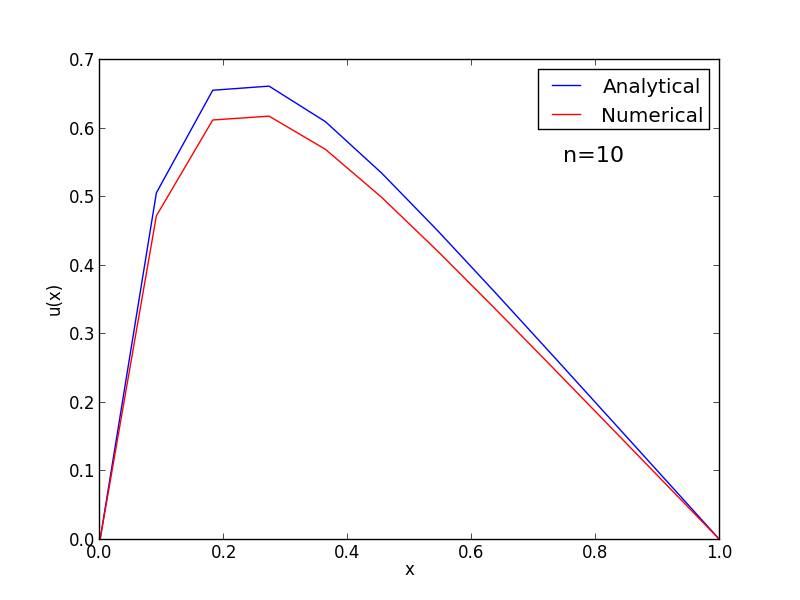
\includegraphics[width=\textwidth]{../plot_n_10.png}
        \caption{}
        %\label{}
  \end{subfigure}
  \begin{subfigure}[b]{0.495\textwidth}
        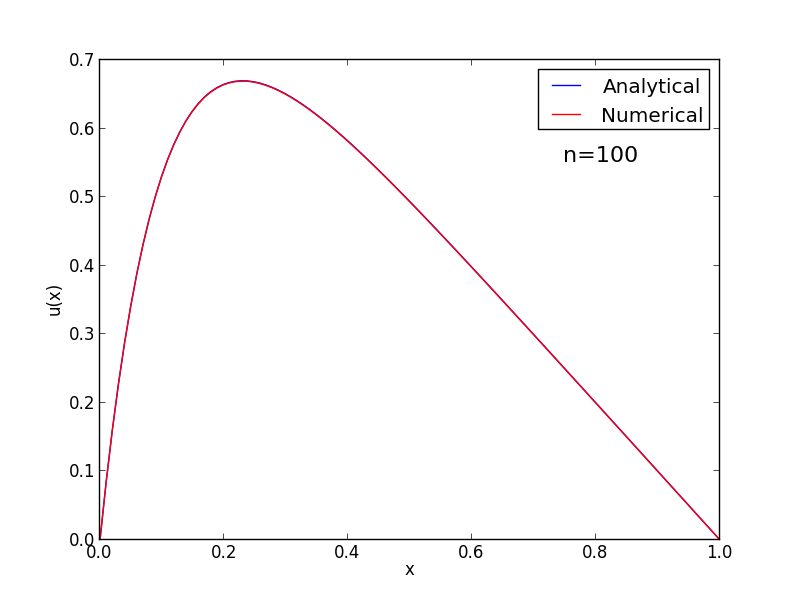
\includegraphics[width=\textwidth]{../plot_n_100.png}
        \caption{}
        %\label{}
  \end{subfigure}
  \begin{subfigure}[b]{0.495\textwidth}
        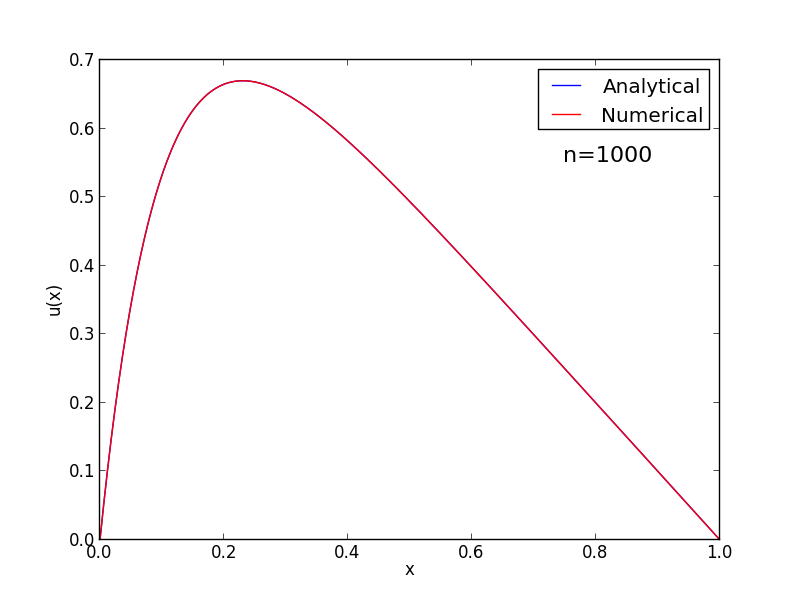
\includegraphics[width=\textwidth]{../plot_n_1000.png}
        \caption{}
        %\label{}
  \end{subfigure}
  \caption{} 
  \label{plots}
\end{figure}

In Table \ref{errors} the $log$-$log$ relation between $h$ and $\epsilon_i$ (defined in eq. 
(\ref{eq:error})) is given. By considering the mathematical truncation error we expect that $\epsilon_i$ 
increases by a factor of $2$ when $n$ is increased by a factor of $10$. We see in the table that this 
holds up to and including $n=10^4$. After this the error seems to be more "random", which must be due to 
limited numerical precision.

\begin{table}[H]
\begin{center}
$\begin{array}{c|c|c} 
n & log_{10}(h) & \epsilon_i \\ \hline 
10^1 & -1.041 & -1.180 \\ 
10^2 & -2.004 & -3.088 \\ 
10^3 & -3.000 & -5.080 \\  
10^4 & -4.000 & -7.079 \\ 
10^5 & -5.000 & -8.843 \\ 
10^6 & -6.000 & -6.075 \\ 
10^7 & -7.000 & -5.525 \\ \hline 
\end{array}$
\end{center}
\caption{}
\label{errors}
\end{table}


\end{document}


